\externaldocument{text-02-teoreticka}
\subsection{Nest watcher}\label{subsec:nest-watcher}
Tato služba interpretuje stavy jednotlivých hnízd v kurníku pro Home Assistanta.
Hlavní funkcí je načítání a analýza dat z jednotlivých vah v hnízdech, která jsou reprezentována Scale Drivery.\newline


Data jsou načítána několikrát do minuty a ukládána do databáze s časovým údajem, kdy byl záznam vytvořen.
Následně se jednou za minutu vyhodnotí průměrná hodnota během posledních několika vážení.
Na základě tohoto údaje jsme schopni zjisti několik případů
\begin{itemize}
    \item hnízdo je prázdné (hodnota na váze nepřevyšuje 50 g )
    \item v hnízdě se nacházejí vejce (hmotnost jednoho vejce je průměrně 50 g)
    \item v hnízdě sedí slepice (hmotnost slepice se pohybuje okolo 1200 g a více)
\end{itemize}
Pokud je na váze průměrně méně než 50 g, vzhledem k možným chybám měření, takový případ vyhodnotíme jako, že je hnízdo prázdné.
Jestliže se hodnota pohybuje mezi 50 a 1200 gramy, znamená to, že v hnízdě jsou pravděpodobně vejce, a jejich počet je vypočítán vydělením celkové hmotnosti a hmotnosti jednoho vejce.
V případě, že je na váze více jak 1200 g, vyhodnotí služba, že v hnízdě sedí slepice.
Tyto tři zmíněné informace služba následně pomocí MQTT předává do Home Assistanta.


Data jsou načítána několikrát za minutu a ukládána do databáze s časovým údajem, kdy byl záznam vytvořen. Následně se jednou za minutu vyhodnotí průměrná hodnota během posledních několika vážení. Tento kontinuální sběr a analýza dat nám umožňuje sledovat a porozumět podmínkám v každém hnízdě v kurníku.

Každý záznam v databázi obsahuje následující strukturu:
\begin{itemize}
    \item \textbf{Časový údaj (timestamp)}: Přesný čas, kdy bylo měření provedeno.
    \item \textbf{ID hnízda (nid)}: Identifikační číslo hnízda (1 až 6), které umožňuje rozlišit mezi jednotlivými hnízdy.
    \item \textbf{Hmotnost (weight)}: Naměřená hmotnost v daném hnízdě v gramech.
    \item \textbf{Stav hnízda (nest\_status)} (volitelné): Automaticky vyhodnocený stav na základě hmotnosti (prázdné, vejce, slepice).
\end{itemize}

Na základě vyhodnocené průměrné hmotnosti jsme schopni zjistit několik případů:
\begin{enumerate}
    \item \textbf{Hnízdo je prázdné}: Pokud průměrná hmotnost nepřevyšuje 50 gramů (vzhledem k možným chybám měření), vyhodnotíme, že hnízdo je prázdné. V hnízdě není ani slepice, ani vejce.
    \item \textbf{V hnízdě se nacházejí vejce}: Jestliže se hodnota hmotnosti pohybuje mezi 50 a 1200 gramy, znamená to, že v hnízdě jsou pravděpodobně vejce. Hmotnost jednoho vejce je přibližně 50 gramů, takže počet vajec lze vypočítat vydělením celkové hmotnosti hmotností jednoho vejce.
    \item \textbf{V hnízdě sedí slepice}: Pokud je průměrná hmotnost na váze více než 1200 gramů, vyhodnotí služba, že v hnízdě sedí slepice. Hmotnost slepice se pohybuje kolem 1200 gramů a více.
\end{enumerate}

Obrázek~\ref{fig:weight_egg_chart_timeline} znázořňuje hodnotu hmotnosti v čase pro hnízdo s id 1.

\begin{figure}[h]
    \centering
    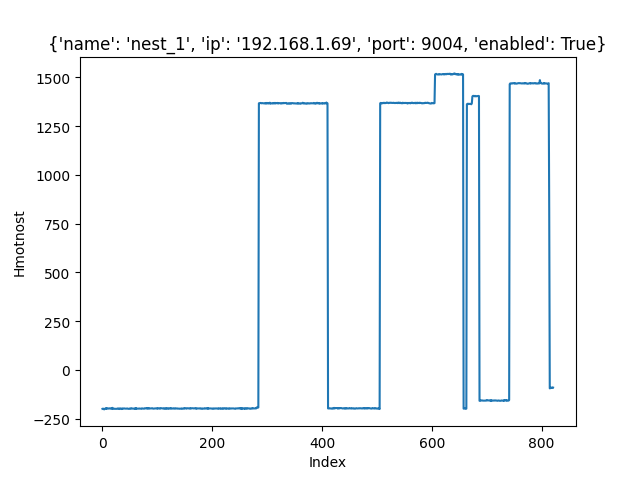
\includegraphics[width=\textwidth]{img/weight_egg_chart_timeline}
    \caption{Proces trénování YOLOv11 modelu}
    \label{fig:weight_egg_chart_timeline}
\end{figure}

Tyto tři zmíněné informace služba následně pomocí MQTT předává do systému Home Assistant pro další zpracování a monitoring. Tím je zajištěna integrace s domácí automatizací a umožněno přijímat notifikace či provádět akce na základě stavu hnízda.

Díky měřením hmotnosti z jednotlivých hnízd můžeme odvodit smysluplné vzorce, které indikují aktuální stav každého hnízda. Kromě výše uvedených případů můžeme z nasbíraných dat identifikovat několik dalších klíčových vzorců:

\begin{enumerate}
    \setcounter{enumi}{3}
    \item \textbf{Doba setrvání slepice v hnízdě}: Analýzou délky období, kdy je hmotnost hnízda nad 1200 gramů, lze zjistit, jak dlouho slepice v hnízdě zůstává. To může poskytnout informace o jejím chování, pohodě a případně upozornit na možné zdravotní problémy, pokud setrvává déle než obvykle.
    \item \textbf{Časové vzorce snášení vajec}: Sledováním časů, kdy dochází ke zvýšení hmotnosti odpovídající snesení vajec, můžeme identifikovat typické doby snášení. To je užitečné pro plánování sběru vajec a optimalizaci péče o slepice.
    \item \textbf{Frekvence snášení u jednotlivých hnízd}: Porovnáním počtu snesených vajec v různých hnízdech lze zjistit, zda některá hnízda nejsou preferována více než jiná. To může vést k úpravám uspořádání kurníku nebo kontrolám hnízd, která jsou méně využívána.
    \item \textbf{Detekce kvokavosti (inkubační chování)}: Pokud slepice setrvává v hnízdě po velmi dlouhou dobu (např. několik hodin či dnů) bez výrazného pohybu, může to indikovat, že začíná kvokat. To je důležité vědět pro správu chovu, neboť kvokavé slepice přestávají snášet vejce.
    \item \textbf{Náhlé změny hmotnosti}: Nečekané nárůsty nebo poklesy hmotnosti mohou upozornit na problémy, jako je zlomené vejce v hnízdě, přítomnost více slepic v jednom hnízdě nebo vstup jiného zvířete. Rychlá reakce na tyto události může zabránit větším komplikacím.
    \item \textbf{Aktivita během noci}: Zaznamenání hmotnosti nad 50 gramů v nočních hodinách může naznačovat neobvyklé chování nebo možné rušení. Slepice by měly v noci odpočívat na bidlech, takže přítomnost v hnízdě může signalizovat stres nebo napadení predátorem.
    \item \textbf{Poruchy senzorů}: Pokud hmotnost zůstává nezměněna po dlouhou dobu nebo vykazuje nerealistické hodnoty, může to indikovat technickou závadu. Pravidelná kontrola a kalibrace senzorů zajistí spolehlivost dat.
    \item \textbf{Denní vzorce aktivity}: Analýzou hmotnostních dat během dne lze určit období nejvyšší aktivity slepic. To může být užitečné pro plánování krmení, čištění kurníku nebo jiných činností, které by mohly slepice rušit.
    \item \textbf{Sledování zdraví slepic}: Dlouhodobé sledování chování slepic může pomoci odhalit zdravotní problémy či změny ve snášce. Například pokles frekvence snášení může být signálem nemoci.
\end{enumerate}

Celkově systém obsluhuje šest hnízd, přičemž každé je nepřetržitě monitorováno a data jsou pravidelně vyhodnocována. Toto komplexní sledování umožňuje efektivní řízení kurníku, zajišťuje optimální péči o slepice a včasný sběr vajec. Přístup založený na datech zvyšuje naši schopnost udržovat zdravé slepice a maximalizovat jejich produktivitu.

\subsection*{Předpokládaná datová struktura v databázi:}

\begin{table}[h!]
\centering
\begin{tabular}{lll}
\textbf{Pole} & \textbf{Datový typ} & \textbf{Popis} \\
timestamp & DATETIME & Datum a čas měření \\
nid & INT & Identifikační číslo hnízda (1 až 6) \\
weight & FLOAT & Naměřená hmotnost v gramech \\
nest\_status & VARCHAR & Stav hnízda (např. "prázdné", "vejce", "slepice") \\
\end{tabular}
\caption{Datová struktura v databázi}
\end{table}

Tato datová struktura umožňuje efektivní ukládání a vyhodnocování dat z jednotlivých hnízd. Pole \texttt{nest\_status} může být automaticky vypočítáno na základě hodnoty v poli \texttt{weight} podle výše uvedených kritérií. Tímto způsobem můžeme snadno filtrovat a analyzovat data pro sledování stavu každého hnízda v čase.

Rozšířená analýza nám poskytuje hlubší vhled do chování slepic a umožňuje nám přijímat informovaná rozhodnutí pro zlepšení podmínek v kurníku, zvýšení produktivity a zajištění pohody zvířat.
